\documentclass[11pt]{article}

\usepackage{color} 
\usepackage{graphics}
\usepackage{graphicx}
\usepackage{pstricks}

\title{\textsf{molsim} tutorial}
\author{J.S. Hansen}
\date{Februaray 2022, v. 0.9}
  
\begin{document}

\maketitle

\section{Introduction}

\textsf{molsim} is a GNU Octave/Matlab toolbox for molecular dynamics simulation
library. \textsf{molsim} supports simulations of
\begin{itemize}
\item standard Lennard-Jones systems,
\item molecular systems with bond, angle, and torsion potentials, 
\item confined flow systems, eg., Couette and Poiseuille flows,
\item charged systems using shifted force and Wolf methods,
\item dissipative particle dynamics systems,
\item and more \ldots
\end{itemize}
The package also supports a series of run-time sampling functionalities.

\bigskip
\noindent \textsf{molsim} is basically a wrapper for the \textsf{seplib}
library, which is a light-weight flexible molecular dynamics simulation library
written in ISO-C99. The library is CPU-based and offers shared memory
parallisation; this parallisaton is supported by the \textsf{molsim}
package. The algorithms used in \textsf{seplib} is based on the books by Allen
\& Tildesley, Rapaport, Frenkel \& Smith, and R. Sadus, see
Ref. \cite{seplib:books}.

\bigskip
\noindent In this text
\begin{verbatim}
>> 
\end{verbatim}
symbolises the GNU Octave/Matlab command prompt. This 
\begin{verbatim}
$ 
\end{verbatim}
symbolises the shell prompt.

\bigskip
\noindent Example scripts to simulate different systems can be found under the
package \textsf{tests} directory.

\section{Installation}
\subsection{GNU Octave}
GNU Octave's package manager offers a very easy installation. From

\begin{verbatim}
https://github.com/jesperschmidthansen/molsim/
\end{verbatim}

\noindent download and save the current release
\verb!molsim-<version>.tar.gz! in a directory of your choice. Start GNU
Octave and if needed change directory to the directory where the file is saved.

\noindent Then type
\begin{verbatim}
>> pkg install molsim-<version>.tar.gz 
\end{verbatim}
to install the package. Check contact by
\begin{verbatim}
>> molsim('hello')
Hello. 
\end{verbatim}
In case this fails, check the path where \textsf{molsim} is install by
\begin{verbatim}
>> pkg list molsim
\end{verbatim}
If the path is not in your GNU Octave search path add this using the
\verb!addpath! command.

\subsection{Matlab}
From
\begin{verbatim}
https://github.com/jesperschmidthansen/seplib/
\end{verbatim}
\noindent download and save the current release \verb!seplib-<version>.tar.gz!
in a directory of your choice. Unpack, configure and build the library
\begin{verbatim}
$ tar zxvf seplib-<version>.tar.gz
$ cd seplib
$ ./configure
$ make
$ cd octave
\end{verbatim}
To build the \textsf{mex}-file enter Matlab
\begin{verbatim}
$ matlab -nodesktop
\end{verbatim}
Then build the 
\begin{verbatim}
>> buildmex
\end{verbatim}
Depending on the system this will build a \textsf{molsim.mex<archtype>}
file. You can copy this file to a directory in your Matlab search path.

\section{First quick example: The Lennard-Jones liquid}
In general, the \verb!molsim! interface is on the form
\begin{verbatim}
molsim(<action>, <specifier>, <arguments>);
\end{verbatim}
where the action can be any particular action the user wishes to perform, for
example, \verb!get!, \verb!calcforce!, \verb!load!, and so on. The action is
further specified by the second argumen; say \verb!lj! specifies that action
\verb!calcforce! should apply the pair-wise Lennard-Jones force. The specifier
arguments are given as the final input.

Listing 1 shows the simplest script simulating a standard Lennard-Jones (LJ)
system in the micro-canonical ensemble where number of particles, volume, and
total energy is conserved. 

\bigskip

\noindent \textbf{Listing 1}
\begin{verbatim}
% Specify the LJ paramters
cutoff = 2.5; epsilon = 1.0; sigma = 1.0; aw=1.0;

% Set init. position and velocities 10x10x10 particles 
% in box with lengths 12x12x12. Velocities set to default. 
% Configuration stored in start.xyz. 
molsim('set', 'lattice', [10 10 10], [12 12 12]);

% Load the configuration file
molsim('load', 'xyz', 'start.xyz');

% Main mol. simulation loop - 10 thousand time steps
for n=1:10000

  % Reset everything
  molsim('reset');

  % Calculate force between particles of type A (default type)
  molsim('calcforce', 'lj', 'AA', cutoff, sigma, epsilon, aw);

  % Integrate forward in time - use leapfrog alogrithm
  molsim('integrate', 'leapfrog');
 
end

% Free memory allocated
molsim('clear');
\end{verbatim}
---

\noindent In Listing 1 information is printed or saved. Inside the main loop you
can add the command
\begin{verbatim}
if rem(n,100)==0
  molsim('print');
end
\end{verbatim}
to print current iteration number, potential energy per particle, kinetic energy
per particle, total energy per particle, kinetic temperature, and total momentum
to screen every 100 time step.

Information can also be stored into variables for further analysis. For example,
to get the system energies and pressure
\begin{verbatim}
[ekin, epot] = molsim('get', 'energies');
press = molsim('get', 'pressure');
\end{verbatim}
and particle positions and velocities
\begin{verbatim}
x = molsim('get', 'positions');
v = molsim('get', 'velocities');
\end{verbatim}

\subsection{NVT and NPT simulations}
Often you will not perform simulations in the microcanonical ensemble, but under
a desired temperature and/or pressure. One way to achieve this with
\verb!molsim! is to use simple relaxation algorithms. To simulate at
temperature, say 2.2, you call the action \verb!'thermostate'! with specifier
\verb!'relax'! after the integration step
\begin{verbatim}
molsim('thermostate', 'relax', 2.2, 0.01);
\end{verbatim}
The last argument is the relaxation parameter; the higher value the faster
relaxation. Notice that too large values makes the system unrealistically
stiff. The best value is optimed via trail-and-error.

To simulate at pressure, say 0.9, you call the action \verb!'barostate'! after
the integration step,
\begin{verbatim}
molsim('barostate', 'relax', 0.9, 0.01);
\end{verbatim}
The choice of relaxation parameter is again a matter of the system. The
barostate works by changing the system box length in the $z$-direction only
(an-isotropic scaling); this is practical when doing sampling as two directions
are fixed. You can use the barostate and the thermostate relaxation actions in
the same simulation mimicking an NPT system.


\section{The \textsf{molsim} force field}
\textsf{molsim} supports simulations of confined, charged, and molecular
systems. In general, the interaction \textsf{molsim} force field is defined from
the potential functional form
\begin{equation}
  U(\mathbf{r}_i, r_{ij}, \ldots)
  =  U_\mathrm{lattice} + U_\mathrm{vWaals} + U_{\mathrm{coloumb}} +
  U_\mathrm{bonds} + U_\mathrm{angles} + 
  U_\mathrm{torsion}
\end{equation}
The first term allows for a simulation of a fictitious fixed crystal
arrangement, where the particles/atoms are tethered around a pre-set lattice
site. The potential function is a harmonic spring type
\begin{equation}
  U_\mathrm{lattice} =
  \sum_\mathrm{sites} \frac{1}{2}k_0 (\mathbf{r}_i - \mathbf{r}_0)^2
\end{equation}
where $k_0$ is the spring constant, $\mathbf{r}_i$ is the position of
particle/atom $i$, and $\mathbf{r}_0$ is the lattice site. The default
lattice site positions are the initial particle positions.

The short ranged van der Waals pair interaction is given via the standard
Lennard-Jones potential
\begin{equation}
  U_\mathrm{vWaals} =  \sum_{i,j \, \mathrm{pairs}}
  4\epsilon\left[\left(\frac{\sigma}{r_{ij}}\right)^{12} - a_w
    \left(\frac{\sigma}{r_{ij}}\right)^{6}\right] \, .
\end{equation}
Here $r_{ij}$ is the particle distance, $\epsilon$ and $\sigma$ define the
characteristic energy and length scales. The parameter $a_w$ determines the
weight of the attractive second term in the potential function.

The Coulomb potential is 
\begin{equation}
  U_{\mathrm{coloumb}} = \sum_{i,j \, \mathrm{pairs}}\frac{q_iq_j}{r_{ij}} \, .
\end{equation}
This long ranged interaction is evaluated using approximative shifted-force or
Wolf methods; this can be specified. These two implementations do not apply to
confined systems.

Particle bonds are model via the harmonic spring potential
\begin{equation}
  U_{\mathrm{bonds}} =\sum_{\mathrm{bonds}} \frac{1}{2} k_{s}(r_{ij} - l_0)^2
\end{equation}
$k_s$ is the spring constant and $l_0$ is the zero force bond length. Note,
currently \textsf{molsim} does not support rigid bonds. 

The angle potential is the cosine squared potential
\begin{equation}
  U_{\mathrm{angles}}=\frac{1}{2}\sum_{\mathrm{angles}} k_{\theta} (\cos(\theta) - \cos(\theta_0))^2 \, ,
\end{equation}
where $k_\theta$ is the force amplitude, and the zero-force angle
$\theta_0$. See Fig. \ref{fig:torsion} for the angle definition.

\begin{figure}[h]
  \begin{center}
    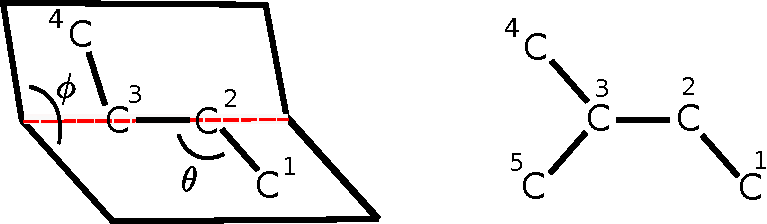
\includegraphics[scale=.7]{diheadral.pdf}
  \caption{
    \label{fig:torsion}
    Illustration of the angle and torsion angle.
  }
  \end{center}
\end{figure}

Finally, the torsion angle potential is the Ryckaert-Belleman potential 
\begin{equation}
  U_\mathrm{dihedral}=\sum_{\mathrm{dihedrals}} \sum_{n=0}^5 c_n
  \cos^n(\pi-\phi)
   \, . 
\end{equation}
Here $c_n$ are the six Ryckaert-Belleman coefficients, and $\phi$ is the
torsion angle, see Fig. \ref{fig:torsion}. Two illustrative 
examples are when $c_n = 0$ except for $n=1$:
\begin{enumerate}
\item If $c_1 > 0$ then the minimum energy torsion angle is $\phi = 0$; this is
  illustrated in the right-hand figure in Fig. \ref{fig:torsion} with torsion
  angle defined by the 1-2-3-5 bonds. Useful for closed molecular ring
  structures.
\item If $c_1 < 0$ then the minimum torsion angle is $\phi = \pi$; this is
  illustrated in the right-hand figure in Fig. \ref{fig:torsion} with
  torsion defined by the 1-2-3-4 bonds. Useful for branched molecular
  structures. 
\end{enumerate}
Below a more complex example is given.

Importantly, you can have different types of particles with different charges,
different bonds, angles, and torsion angles, all determined from the interaction
parameters. It is thus possible to simulate mixtures, highly complex molecules,
etc.

\section{Molecular systems: Toluene}
This example shows how to setup a simulation of model liquid toluene. The model
of the molecule is a united atomic unit (UAU) model. This means that each carbon
group is represented by a single Lennard-Jones particle, thus, the toluene
molecule is composed of seven Lennard-Jones particles, six forming the phenyl
ring structure (index 2-7) and one representing the -CH$_3$ group (index 1), see
Fig. \ref{fig:toluene}.
\begin{figure}[h]
  \begin{center}
    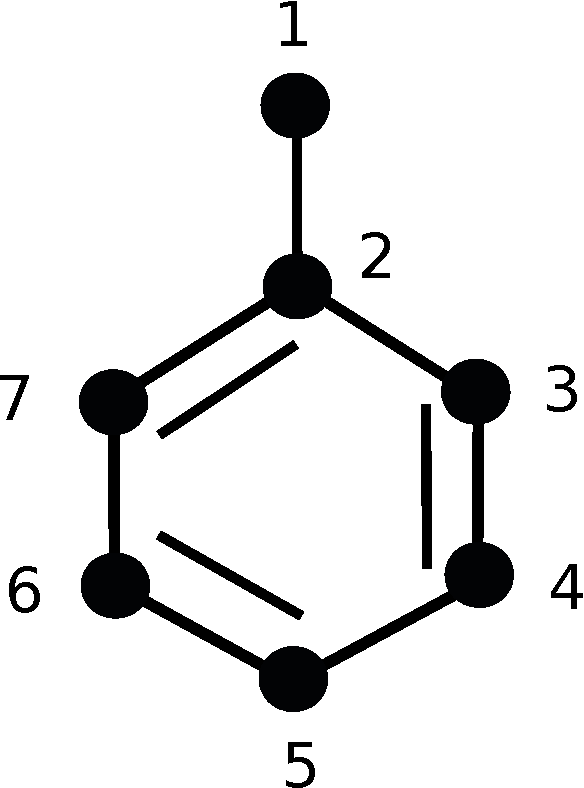
\includegraphics[scale=.4]{toluene.pdf}
  \caption{
    \label{fig:toluene}
    United atomic unit representation of toluene.
  }
  \end{center}
\end{figure}

The intra-molecular interactions are given through bond, angle, and torsion
angle potentials; Lennard-Jones interactions between carbon groups in same
molecule are excluded. The model is further simplifed by using only two bonds
and one angle interaction. There are two different torsion angles, eg., 1-2-3-4
form one type of torsion angle, $\phi=\pi$, whereas 7-2-3-4 is an example of the
other torsion angle with $\phi=0$. We define the molecular model in two files;
one with extension \verb!.xyz! giving UAU positions for the molecule and one with
extension \verb!.top! defining bonds and angles in the molecule. You can find
examples of these two files for different molecules under the \verb!resources!
directory. To setup the entire system (i.e. the ensemble of molecules) we copy the
single molecule \verb!.xyz! and \verb!.top! to the current directory and use the
\verb!set! action; for example to simulate 500 molecules
\begin{verbatim}
>> molsim('set', 'molconfig', 'toluene.xyz', 'toluene.top', ... 
   500, 0.05, 42)
\end{verbatim}
The two last arguments are the molecular number density (keep very low initially
and compress the system afterwards), and a seed for the random number
generator. This generates a system \verb!start.xyz! file and \verb!start.top!
file. 

We now only need the parameter values for the interaction potentials and we will
simply take what is available in the literature and convert them into MD reduced
units. Listing 2 shows the resulting script

\bigskip

\noindent \textbf{Listing 2}
\begin{verbatim}
% Simulation parameters
temp0 = 4.0; dens0 = 1.95; dt  = 0.001; nloops = 200000;

% Intra-molecular parameters
bondlength_0 = 0.4; bondlength_1 = 0.38; springconstant = 48910;
bondangle = 2.09; angleconstant = 1173;

torsionparam_0 = [0.0, 133.0, 0.0 0.0 0.0]; 
torsionparam_1 = [0.0, -133.0, 0.0 0.0 0.0];

% Load positions, set temp, remove intra-molecular pair-interaction etc
molsim('load', 'xyz', 'start.xyz');
molsim('load', 'top', 'start.top');

molsim('set','timestep', dt);
molsim('set', 'temperature', temp0);
molsim('set', 'exclusion', 'molecule');

% Main loop
for n=1:nloops
  molsim('reset')

  molsim(’calcforce’, ’lj’, ’CC’, 2.5, 1.0, 1.0, 1.0);
  
  molsim(’calcforce’, ’bond’, 0, bondlength_0, springconstant);
  molsim(’calcforce’, ’bond’, 1, bondlength_1, springconstant);
  
  molsim(’calcforce’, ’angle’, 0, bondangle, angleconstant);

  molsim(’calcforce’, ’torsion’, 0, torsionparam_0);
  molsim(’calcforce’, ’torsion’, 1, torsionparam_1);
  
  molsim('thermostate', 'nosehoover', 'C', temp0, 10.0);
  molsim('integrate', 'leapfrog');

  molsim('compress', dens0);

end
\end{verbatim}

\noindent ---

\noindent Note, the bond and angle types are specified through the third
argument.  

\section{Sampling}
The user can access the system configuration through the \verb!get! action and
from this perform data analysis via GNU Octave's or Matlab's built-in
tools. \textsf{molsim} also offers some runtime data sampling. The different
samplers can be initialised before the main loop using the \verb!sample! action
\begin{verbatim}
molsim('sample', <sample specifier>, <arguments>);
\end{verbatim}
For example, to sample the stress autocorrelation function with 200 sample points
and over a sample time span window of 5.0 we write
\begin{verbatim}
molsim('sample', 'sacf', 200, 5.0);
\end{verbatim}
The actual sampling is carried out by the specifier \verb!do!, and in the main
loop there must be the call
\begin{verbatim}
molsim('sample', 'do'); 
\end{verbatim}
Typically this call is done just after the integration call. Check the reference
sheet for the list of available samplers. 

\section{The two parallisation paradigms}
\textsf{molsim} offers two types of sheared memory parallisation methods,
namely,  
\begin{itemize}
\item Loop parallisation n in force calculations
\item Task-block parallisation
\end{itemize}
To use the first method simply use the \verb!set! action
\begin{verbatim}
molsim('set', 'omp', <nthreads>);
\end{verbatim}
where \verb!nthreads! is the number of threads you will use. The call is placed
anywhere before the main loop. Be aware that depending on your hardware and the
particular system the parallelisation efficiency quickly drop as function of
number of threads. Fig. \ref{fig:bench} shows an example of a benchmark for a
simple Lennard-Jones system.  


\appendix

\clearpage
\begin{center}
  
  \begin{tabular}{cclclcccc}
    {\color{red}{\textbf{Action}}} && {\color{blue}{Specifier}} && Arguments && Output \\
                                   && && && \\
    \hline
                                   && && && \\
    \verb!load! && \verb!xyz! && file name && \\
    $\mbox{}$ && \verb!top! && file name && \\
                                   && && && \\
    \hline
    && && && \\
    \verb!save! &&  && 1: type names && \\
                &&  && 2: file name && \\
                                   && && && \\
    \hline
                                   && && && \\
    \verb!set! && \verb!timestep! && time step (0.005) && \\
    $\mbox{}$  && \verb!temperature! && temperature (1.0) && \\
    $\mbox{}$  && \verb!cutoff! && Max. cut-off (2.5) && \\
    $\mbox{}$  && \verb!omp! && No. of threads && \\
    $\mbox{}$ && \verb!exclusion! && 'bonded' or 'molecule' && \\
    $\mbox{}$ && \verb!temperaturerelax! && relaxation time (0.01) && \\
    $\mbox{}$ && \verb!compressionfactor! && compress factor && \\
    $\mbox{}$ && \verb!types! && particles types (vector string) && \\
    $\mbox{}$ && \verb!skin! && buffer-skin neighblist && \\
    $\mbox{}$ && \verb!charges! && atom charges (vector) && \\
    $\mbox{}$ && \verb!lattice! && 1: array $N_x , N_y , N_z$ && \\
    $\mbox{}$ && $\mbox{}$      && 2: array $L_x, L_y, L_z$ && \\
  \end{tabular}

\end{center}
\end{document}
